\documentclass[aspectratio=169]{beamer}
\beamertemplatenavigationsymbolsempty
\usecolortheme{beaver}
\setbeamertemplate{blocks}[rounded=true, shadow=true]
\setbeamertemplate{footline}[page number]
%
\usepackage[utf8]{inputenc}
\usepackage[english]{babel} % Removed Russian
\usepackage{amssymb,amsfonts,amsmath,mathtext}
\usepackage{booktabs}
\usepackage{subfig}
\usepackage[all]{xy} % xy package for diagrams
\usepackage{array}
\usepackage{tikz}
\usepackage{multicol}% many columns in slide
\usepackage{hyperref}% urls
\usepackage{hhline}%tables
% Your figures are here:
\graphicspath{ {fig/} {../fig/} }

\newcommand\argmin{\mathop{\arg\min}}
% \newcommand{\T}{^{\text{\tiny\sffamily\upshape\mdseries T}}}
\newcommand{\hchi}{\hat{\boldsymbol{\chi}}}
\newcommand{\hphi}{\hat{\boldsymbol{\varphi}}}
\newcommand{\bchi}{\boldsymbol{\chi}}
\newcommand{\A}{\mathbf{A}}
\newcommand{\bb}{\mathbf{b}}
\newcommand{\B}{\mathcal{B}}
\newcommand{\T}{\mathcal{T}}
\newcommand{\W}{\mathbf{W}}
\newcommand{\E}{\mathbb{E}}
\newcommand{\V}{\mathbb{V}}
\newcommand{\x}{\mathbf{x}}
\newcommand{\y}{\mathbf{y}}
\newcommand{\Y}{\mathbf{Y}}
\newcommand{\X}{\mathbf{X}}
\newcommand{\Z}{\mathbf{Z}}
\newcommand{\hx}{\hat{x}}
\newcommand{\hX}{\hat{\X}}
\newcommand{\hy}{\hat{y}}
\newcommand{\M}{\mathcal{M}}
\newcommand{\N}{\mathcal{N}}
\newcommand{\R}{\mathbb{R}}
\newcommand{\p}{p(\cdot)}
\newcommand{\cc}{\mathbf{c}}
\newcommand{\m}{\mathbf{m}}
\newcommand{\bt}{\mathbf{t}}
\newcommand{\e}{\mathbf{e}}
\newcommand{\h}{\mathbf{h}}
\newcommand{\q}{q(\cdot)}
\newcommand{\uu}{\mathbf{u}}
\newcommand{\vv}{\mathbf{v}}
\newcommand{\dd}{\partial}
\renewcommand{\S}{\mathcal{S}}

\newtheorem{Th}{Theorem} % Changed from Russian

%----------------------------------------------------------------------------------------------------------
\title[\hbox to 56mm]{Automatic Hierarchical Summarization of Scientific Texts} % Translated title
\author[Fedor Alexandrovich Sobolevsky]{Fedor Alexandrovich Sobolevsky\\Scientific supervisor~--- D.\,Sc. Konstantin Vyacheslavovich Vorontsov} % Translated author
\institute{Moscow Institute of Physics and Technology} % Translated institute
\date{2025}

%%%%%%%%%%%%%%%%%%%%%%%%%%%%%%%%%%%%%%%%%%%%%%%%%%%%%%%%%%%%%%%%%%%%%%%%%%

\begin{document}

%%%%%%%%%%%%%%%%%%%%%%%%%%%%%%%%%%%%%%%%%%%%%%%%%%%%%%%%%%%%%%%%%%%%%%%%%%

\maketitle

%%%%%%%%%%%%%%%%%%%%%%%%%%%%%%%%%%%%%%%%%%%%%%%%%%%%%%%%%%%%%%%%%%%%%%%%%%

\begin{frame}{Problem Statement}
\begin{columns}
\column{0.5\linewidth}
    
A \textbf{hierarchical summary} is a summary of a document in the form of a \textbf{text tree}~--- a tree $T = (V, E)$, where $E \subset V^2$ and for each $v\in V$ a text $s(v)\in\mathcal{S}$ is defined.

\textbf{Hierarchical summarization problem:} Find a mapping $f: D\mapsto T$ that constructs a hierarchical summary $T\in\mathcal{T}$ from a document $D$, minimally different from a reference summary $T^*$ of $D$ constructed by an expert:
$$
\rho(f(D), T^*)\longrightarrow\min_f.
$$

\column{0.5\linewidth}
    \centering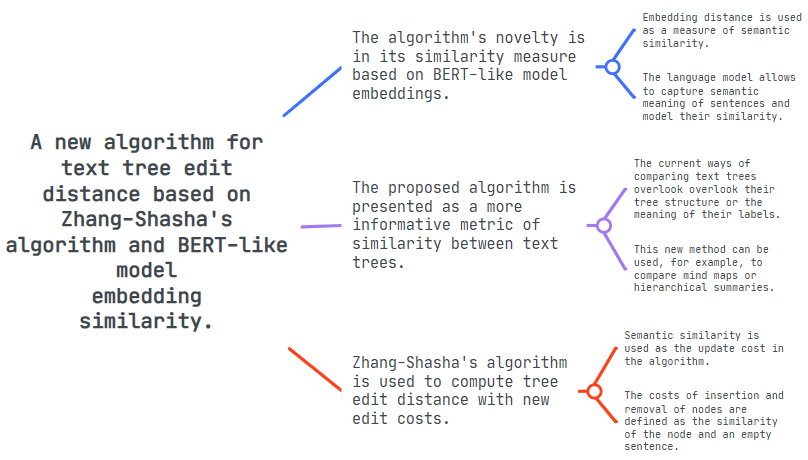
\includegraphics[width=\linewidth]{img/map_example.png}
    \scriptsize
    An example of a hierarchical summary of this study

\end{columns}

\end{frame}

%%%%%%%%%%%%%%%%%%%%%%%%%%%%%%%%%%%%%%%%%%%%%%%%%%%%%%%%%%%%%%%%%%%%%%%%%%

\begin{frame}{Problem Statement}

The following requirements for hierarchical summaries are introduced:
\begin{enumerate}
    \item \textbf{Completeness:} a hierarchical summary, expanded to an arbitrary depth, is a complete summary of the source document.
    \item \textbf{Conciseness:} a hierarchical summary, expanded to an arbitrary depth, should be concise, i.\,e. it should present information from the source document in as brief of a way as possible without losing any relevant information. 
    \item \textbf{Coherence:} a hierarchical summary, expanded to an arbitrary depth, should be coherent when read in depth-first order. 
\end{enumerate}

\end{frame}

%%%%%%%%%%%%%%%%%%%%%%%%%%%%%%%%%%%%%%%%%%%%%%%%%%%%%%%%%%%%%%%%%%%%%%%%%%

\begin{frame}{Metrics}
\begin{columns}
\column{0.6\linewidth}

Baseline metric~--- \textbf{TTED}\footnote{\textit{Sobolevsky, Fedor and Vorontsov, Konstantin.} Text Tree Edit Distance: A Language Model-Based Metric for Text Hierarchies (2025)}.
\vspace{5pt}

Modifications:
\begin{enumerate}
    \item Normalization\footnote{\textit{Li, Yujian and Chenguang, Zhang.} A metric normalization of tree edit distance}:
    $$
        \text{nTTED}(T_1, T_2) = \frac{2\cdot \text{TTED}(T_1, T_2)}{|T_1| + |T_2| + \text{TTED}(T_1, T_2)};
    $$

    \item Comparison at depth $k$:
    $$
    \text{TTED}@k(T_1, T_2) = \text{TTED}(T_1@k, T_2@k),
    $$
\end{enumerate}

\column{0.4\linewidth}
    \centering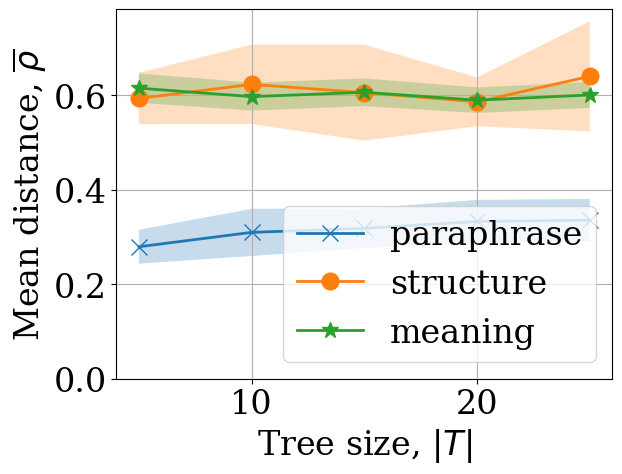
\includegraphics[width=\linewidth]{img/mpnet_graph_avg.png}
    \scriptsize
    Scores by nTTED are tree size-agnostic yet still reflect significant differences the most

\end{columns}

\end{frame}

%%%%%%%%%%%%%%%%%%%%%%%%%%%%%%%%%%%%%%%%%%%%%%%%%%%%%%%%%%%%%%%%%%%%%%%%%%

\begin{frame}{Method: LLM Generation}
\begin{columns}
\column{0.5\linewidth}

The method for automatic hierarchical summary generation in this study is by using \textbf{large language models (LLMs)}.
\vspace{5pt}

\textbf{Proof-of-concept experiment}~--- comparison of LLM mind map generation against SoTA graph-based methods\footnote{\textit{Zhang Zhuowei, Hu Mengting, Bai Yinhao, and Zhang Zhen.} Coreference Graph Guidance for Mind-Map Generation (2024)}. Similarity function based on R~--- ROUGE (as in other studies):
$$
\text{Sim}(T, T') = \max\limits_{P\subset E\times E'} \sum\limits_{(e, e')\in P}\sum\limits_{i=0,1}\text{R}(e_i, e'_i).
$$

\column{0.5\linewidth}
    \centering
    \begin{tabular}{c|cccc}
        \toprule
        \textbf{Models} & \textbf{Sim} \\
        \midrule
        Random & 28.77 \\
        MRDMF & 34.47 \\
        EMGN & 42.73 \\
        CMGN & 44.27 \\
        \midrule
        Qwen2.5-3B-Instruct (1-shot) & 41.58 \\
        Qwen3-4B-Instruct (1-shot) & \textbf{46.83} \\
        \bottomrule
    \end{tabular}
    
    \vspace{5pt}
    \scriptsize
    Mind map generation results. Even a small modern LLM can outperform graph-based methods with good prompting.

\end{columns}

\end{frame}

%%%%%%%%%%%%%%%%%%%%%%%%%%%%%%%%%%%%%%%%%%%%%%%%%%%%%%%%%%%%%%%%%%%%%%%%%%

\begin{frame}{LLM Evaluation}
\begin{columns}
\column{0.33\linewidth}
    \centering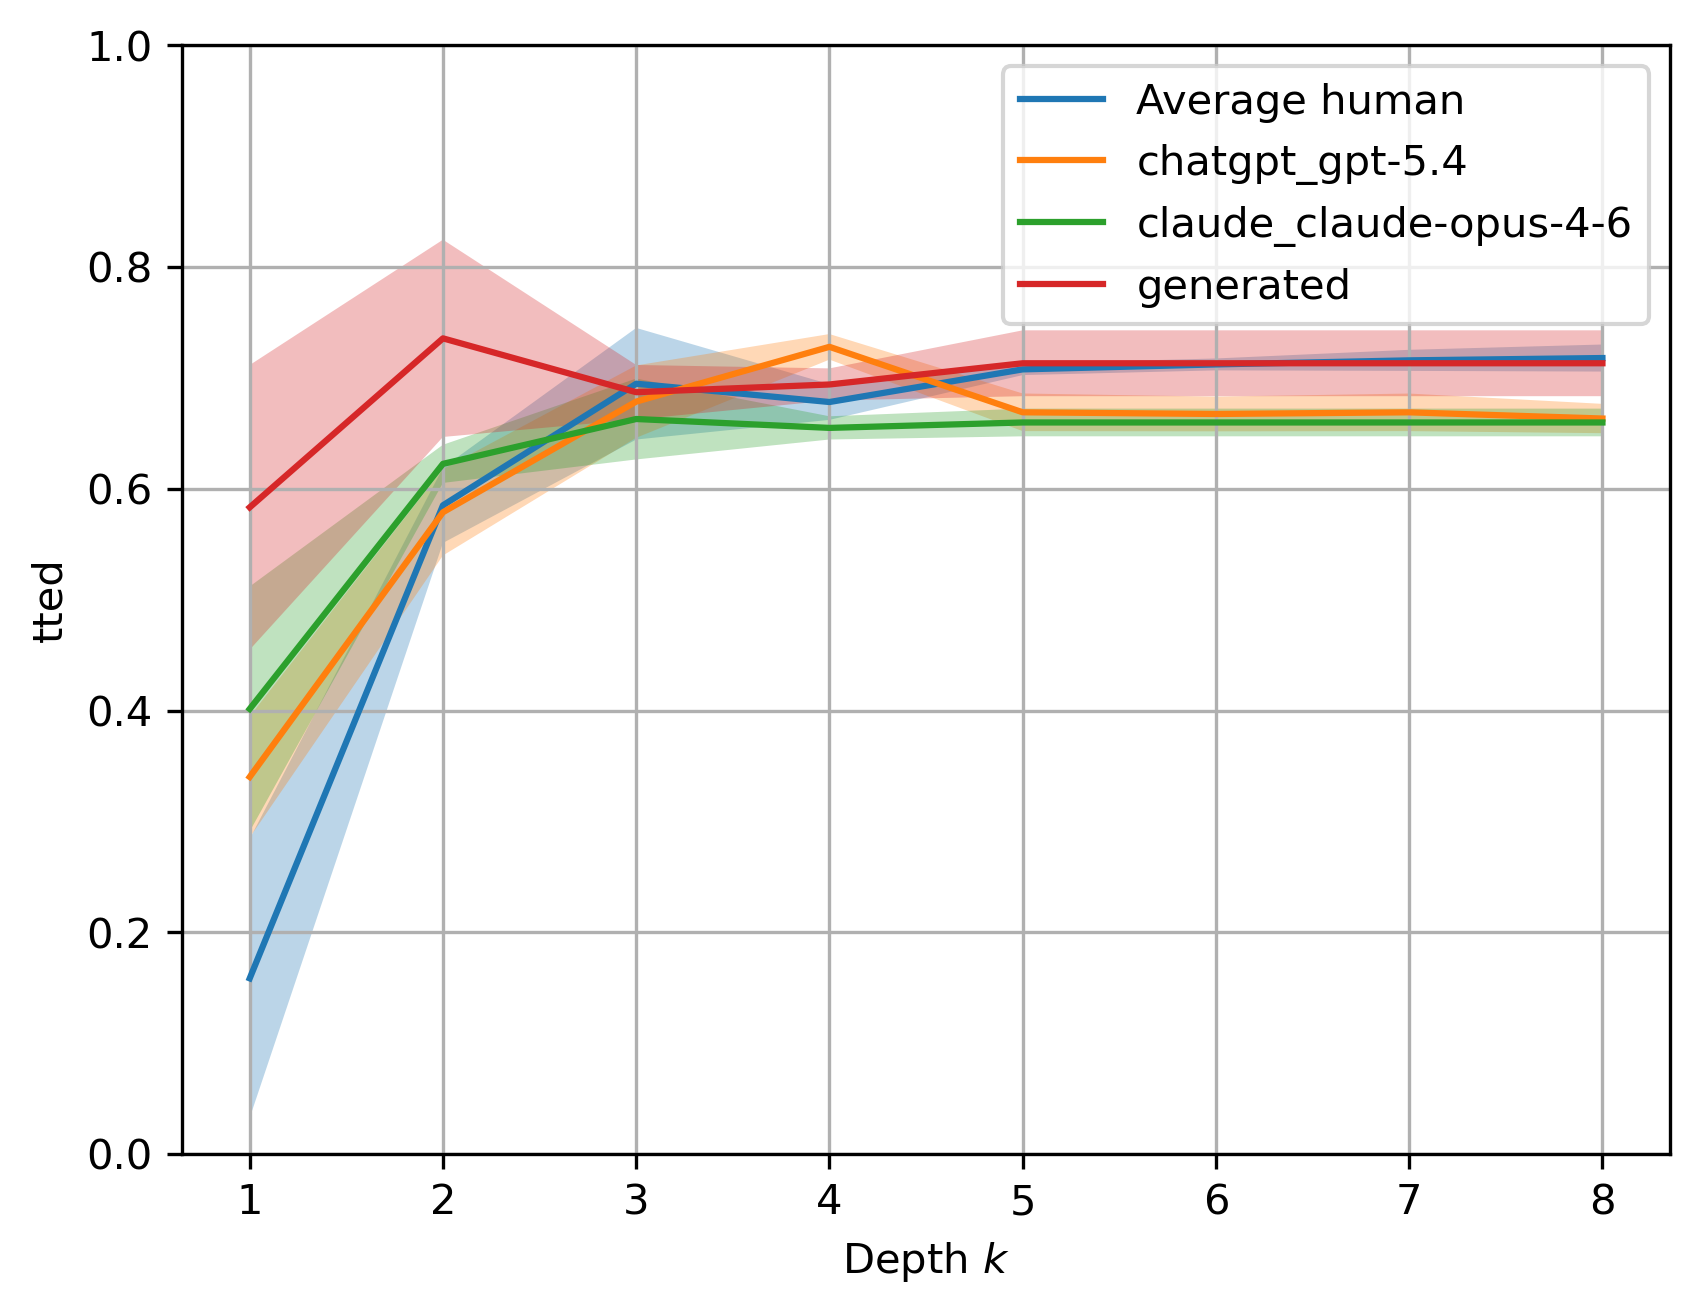
\includegraphics[width=\linewidth]{img/tted.png}
    \scriptsize
    TTED
\column{0.33\linewidth}
    \centering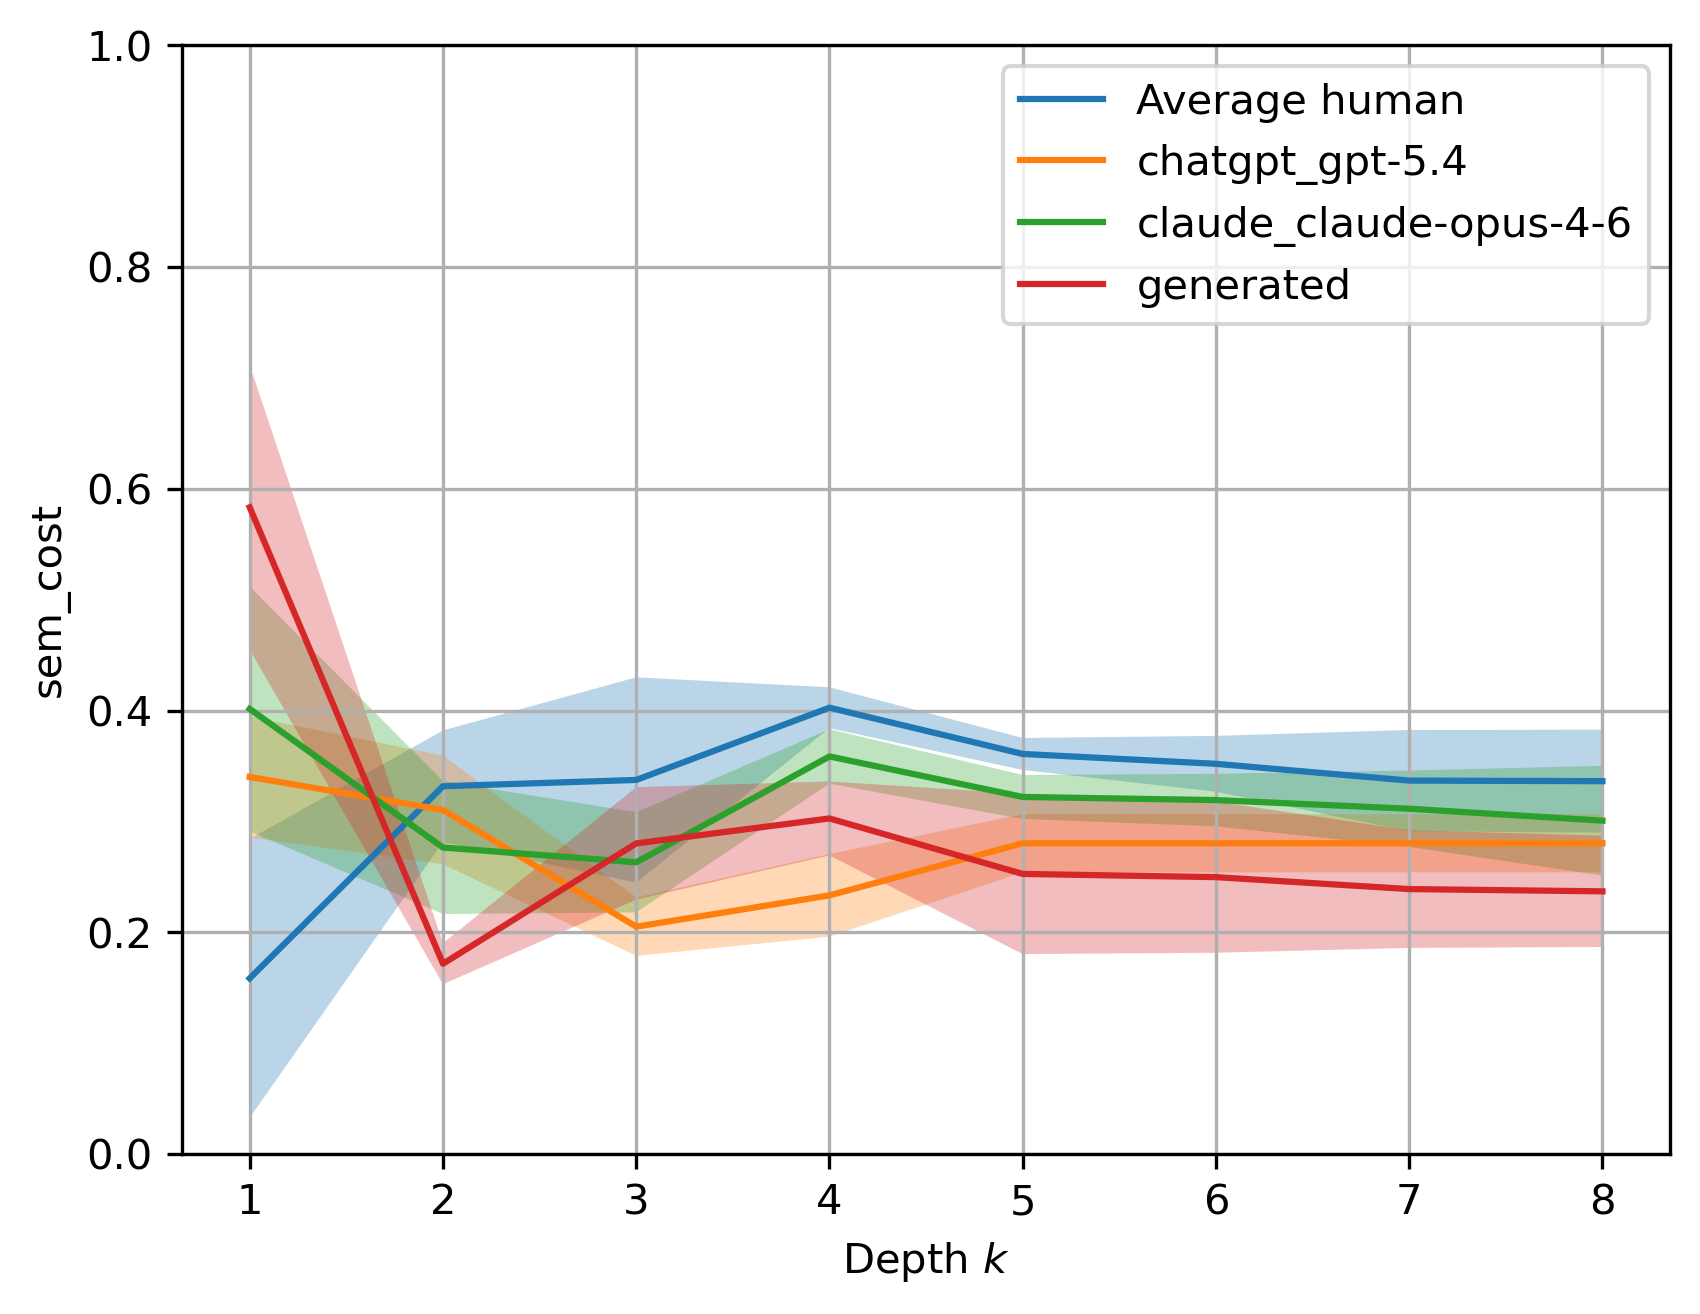
\includegraphics[width=\linewidth]{img/sem_cost.png}
    \scriptsize
    Semantic component of TTED
\column{0.33\linewidth}
    \centering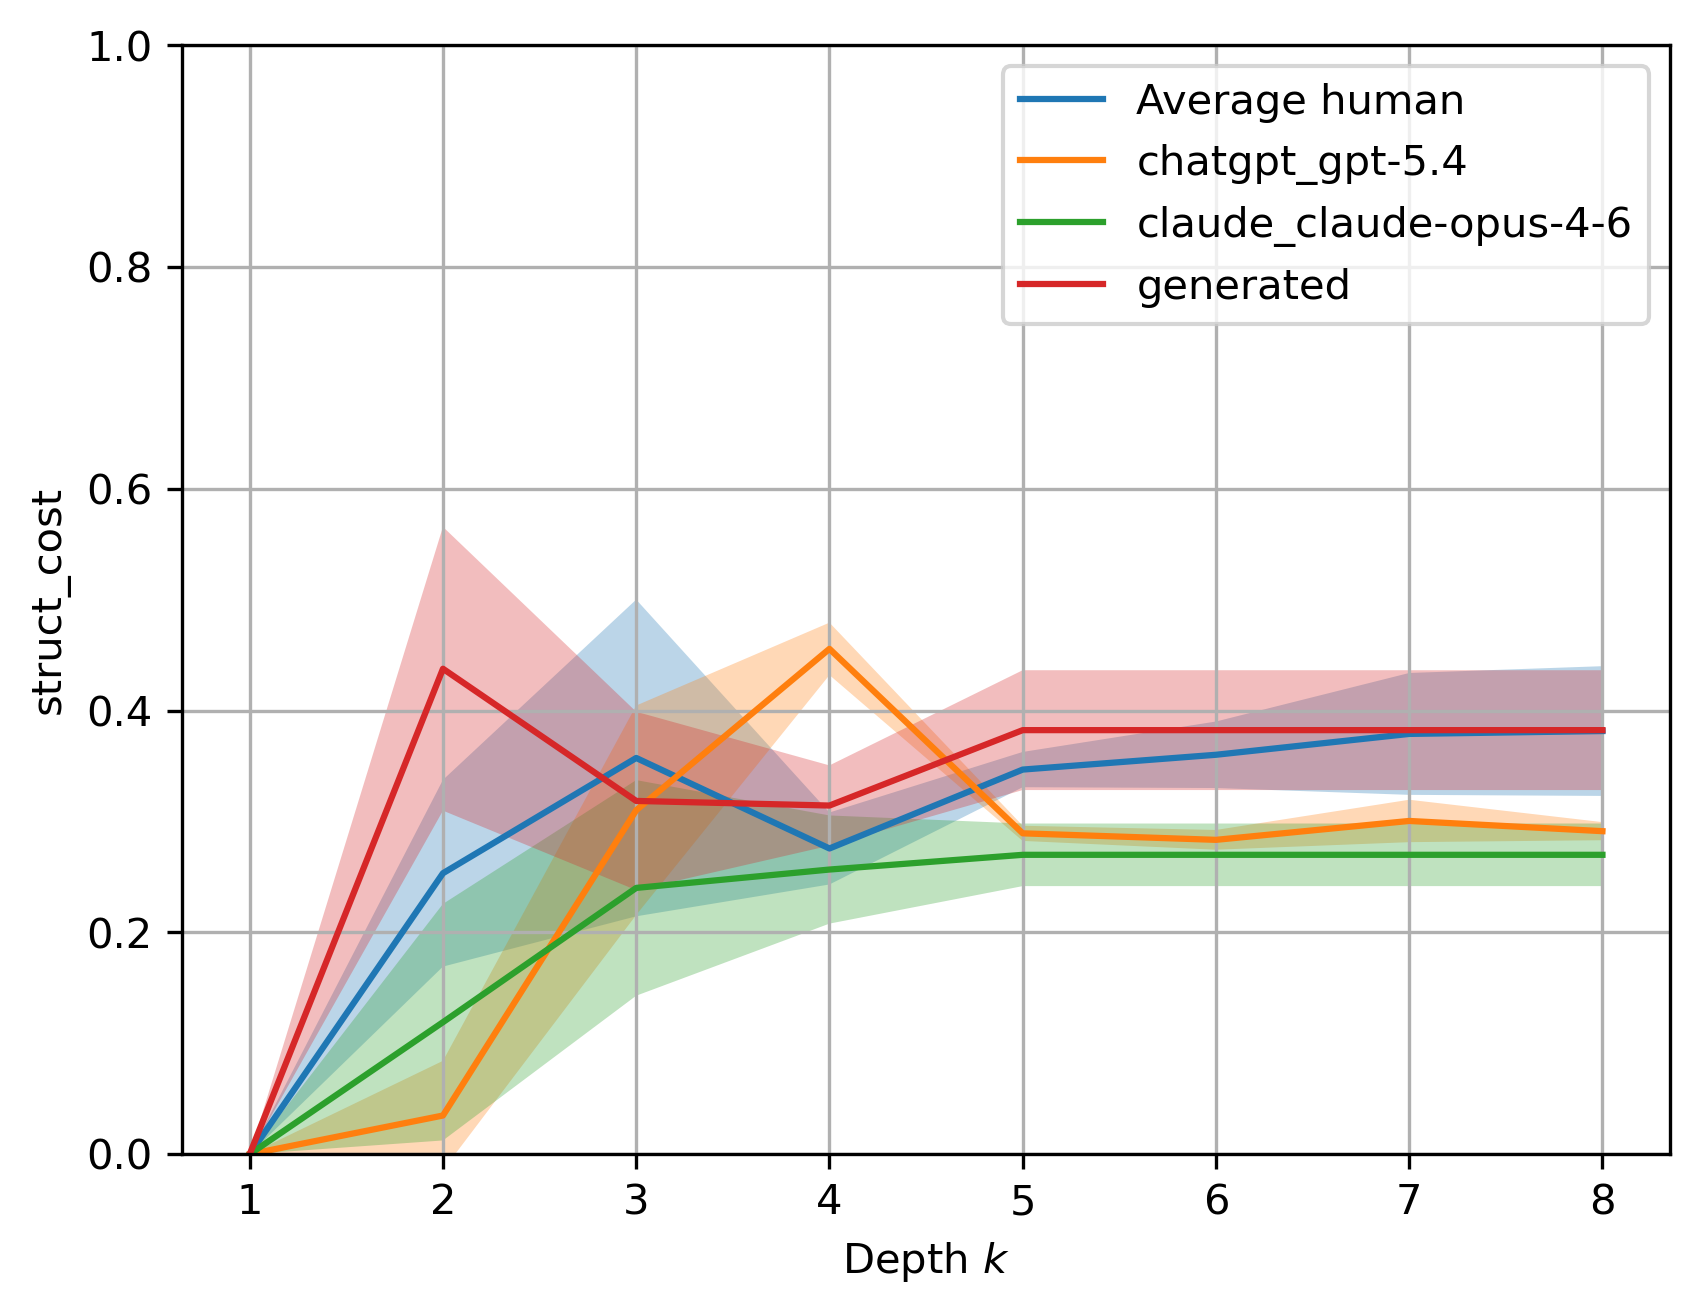
\includegraphics[width=\linewidth]{img/struct_cost.png}
    \scriptsize
    Structural component of TTED

\end{columns}
\vspace{10pt}

\centering
The results of LLM evaluation on a human hierarchical summary benchmark show that difference between LLM generated hierarchical summaries and references is on average not higher than between references.


\end{frame}
%%%%%%%%%%%%%%%%%%%%%%%%%%%%%%%%%%%%%%%%%%%%%%%%%%%%%%%%%%%%%%%%%%%%%%%%%%


\begin{frame}{Main Results}

\begin{enumerate}
    \item The requirements for a quality hierarchical summary have been formalized.
    \item TTED modifications have been proposed for more flexible and interpretable summary comparison.
    \item Small LLMs have been shown to outperform SoTA methods for mind map generation.
    \item An evaluation framework has been built for the task of hierarchical summarization.
    \item First results have been acquired for LLM evaluation on a human hierarchical summary benchmark.
\end{enumerate}

\end{frame}

%%%%%%%%%%%%%%%%%%%%%%%%%%%%%%%%%%%%%%%%%%%%%%%%%%%%%%%%%%%%%%%%%%%%%%%%%%%%

\begin{frame}{References}

\begin{itemize}
    \item \textit{Sobolevsky, F. and Vorontsov, K.} 2025. Text tree edit distance: A language model-based metric for text hierarchies. In 2025 IEEE XVII International Scientific and Technical Conference on Actual Problems of Electronic Instrument Engineering (APEIE), pages 1–5. IEEE.
    \item \textit{Zhang, Z., Hu, M., et al.} 2024. Coreference Graph Guidance for Mind-Map Generation // Proceedings of the AAAI Conference on Artificial Intelligence. — Vol. 38. — P. 19623–19631.
    \item \textit{Li, Y. and Chenguang, Z.} 2011. A metric normalization of tree edit distance. Frontiers of Computer Science in China, 5(1), pp. 119-125.
\end{itemize}

\end{frame}

%%%%%%%%%%%%%%%%%%%%%%%%%%%%%%%%%%%%%%%%%%%%%%%%%%%%%%%%%%%%%%%%%%%%%%%%%%



\end{document}